\documentclass[a4paper,12pt,english]{all-in-one} %% TWOSIDE
\usepackage{amsmath} 
\usepackage{newtxmath}
\usepackage{multicol}
\usepackage{lipsum}
\usepackage{subfig}
\usepackage{listings}
\usepackage[hidelinks]{hyperref}
\renewcommand\theequation{\arabic{equation}}
\newcommand\tab[1][1cm]{\hspace*{#1}} 

\doctitle{Modern Physics Laboratory }
\docsubtitle{Compton effect} % Experiment name here

\makeatletter
\title{{\large\textit{Modern Physics Laboratory | PHYS-461}}\\[0.5cm]{\Huge\color{gray}\textsc{\@docsubtitle}}}
\makeatother

\author{\textbf{Cordney Nash}  \and Micah Hillman  }
\date{November 13, 2024}
\footext{}



\begin{document}

\begin{titlepage}
\maketitle\vfill
\end{titlepage}
\newpage


\section*{Introduction}
{
In the Compton effect, an incoming photon collides elastically with an electron, resulting in the scattering of the photon with altered momentum and direction. The theory behind Compton scattering combines principles of relativistic and quantum mechanics, as it deals with massless photons and involves substantial energy transfers relative to the electron’s rest energy. While the Compton effect applies to photons of various energies, including visible light, this experiment focuses on higher-energy photons, specifically gamma rays, to observe and analyze the effect more clearly. In the end, we wish to determine the rest energy $E_0$ of the electron.
}

\begin{figure}[tbh]
    \centering
    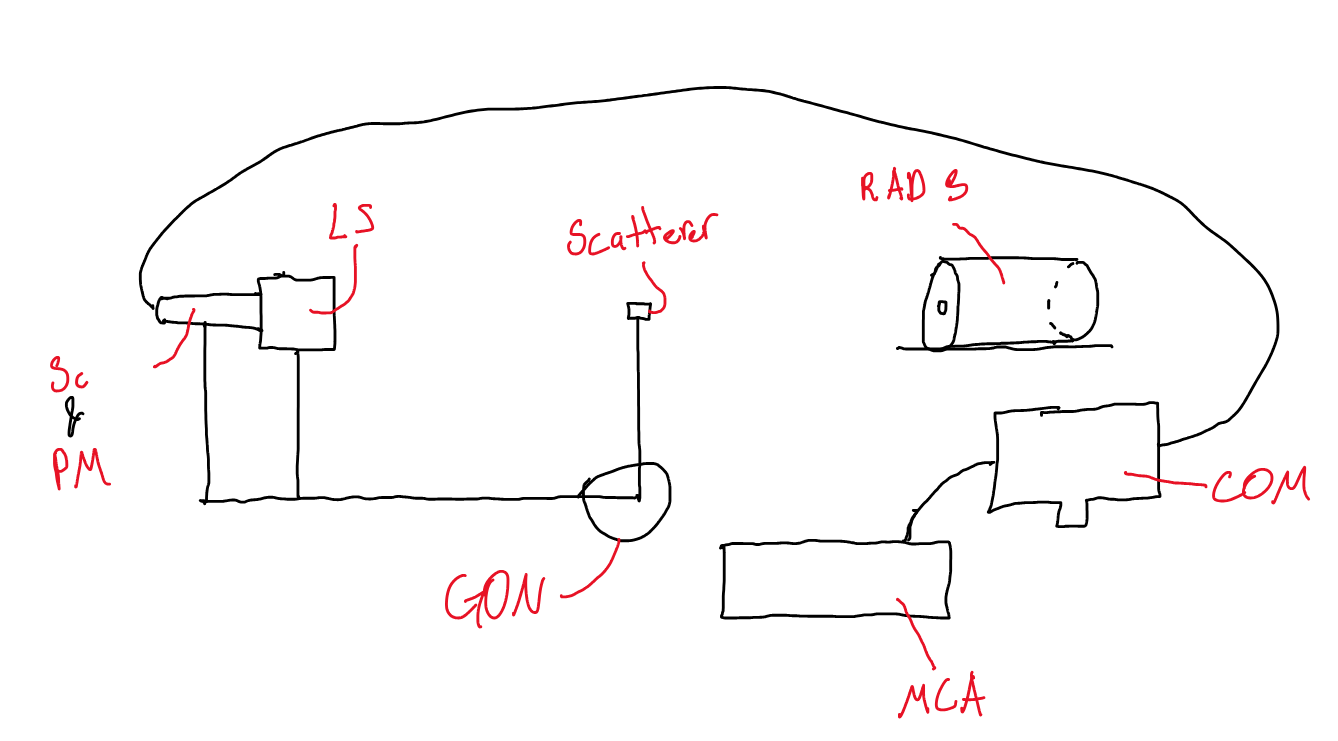
\includegraphics[width=0.8\linewidth]{6-compton/images/Screenshot from 2024-11-16 17-29-02.png}
    \caption{  Lead Shielding (LS), Scintillator (SC) \& Photon Multiplier (PM), Goniometer (GON), Radiation Source (RAD S), Multichannel Analyzer (MCA), Computer (COM).
    }
    \label{fig:compton-diagram}
\end{figure}

\begin{multicols}{2}

\section*{Theory \& Procedure}
{
When interacting with a stationary electron, a photon transfers energy and momentum through an elastic collision. The photon scatters at an angle $\theta$, moving with lower energy and momentum, while the electron gains kinetic energy. This phenomenon is governed by the laws of energy and momentum conservation. Due to the high-energy nature of the incoming gamma rays and their interactions, this process is framed within the context of relativistic mechanics. Also, it negates the effects observed in the photoelectric effect and pair production. In the case of pair production, high-energy gamma rays are required to meet a threshold of approximately 1020 keV. However, the gamma rays used in this experiment have an energy of 622 keV. Regarding the photoelectric effect, when a photon impacts the material, most of its energy is converted into the kinetic energy of the electron. This energy dissipates quickly within the material, making it difficult to study the electron. In Compton scattering, gamma rays with an energy of 622 keV make this the most probable process

When producing the gamma rays used in this experiment, we use a Cesium-137 ($Cs-137$) source. This $Cs-137$ source experienced beta radiation, meaning it decayed into Barium-137 ($Ba-137$). From here, the $Ba-137$ source decays into the ground state by emitting a 662 $keV$ photon, which is the energy of a gamma ray.


When trying to relate a scattered photon's energy to its initial energy and scattering angle we can use  Compton's equation,

\begin{equation}
    \frac{1}{E_0}[1-cos(\theta)] = \frac{1}{E'} - \frac{1}{E}
\end{equation}
where $\theta$ is the scattering angle, $E_0$ is the electron's rest energy, $E$ is the initial photon energy, and $E'$ is the energy of the scattered photon. This equation shows that the photon's energy loss depends on the scattering angle and the rest energy of the particle it interacts with. The maximum energy transfer to the electron corresponds to a scattering angle of $\theta$ = 180$^\circ$, while smaller $\theta$ correspond to less energy being transferred.

At the heart of the detection process is the scintillation detector, which consists of a sodium iodide ($NaI$) crystal coupled to a photomultiplier tube (PMT). When a gamma ray interacts with the NaI crystal, it produces a flash of visible light (scintillation). This light is converted into electrons by the PMT’s photocathode, and these electrons are multiplied through a series of dynodes in the PMT, resulting in a measurable electric signal. The size of this signal is proportional to the energy deposited in the detector by the gamma ray, enabling energy analysis of scattered photons.

To record and analyze the signals, a multichannel analyzer (MCA) is used. The MCA sorts the electric signals into channels based on their voltage, which corresponds to the gamma ray’s energy. This allows the energy spectrum to be measured. A goniometer setup enables precise positioning of the detector at various scattering angles relative to the source and target. These components, combined with a computer-controlled DAQ system, allow for detailed measurement and analysis of the scattered gamma rays.

The first step in starting the experiment is to open the UCS-30 MCA software and correctly calibrate the system. This is done with the Cesium-137 ($Cs-137$) source along with a Sodium-22 ($Na-22$) radiation source. To effectively calibrate we need three peaks: the first two, 662 $keV$ and 32 $keV$, are found from $Cs-137$ and the third point at 511 $keV$ is found from $Na-22$. This calibration is done each day we decide to take measurements. We must also be sure that the High Voltage is set to 850, the Coarse Gain is set to 16 and, Fine Gain is shifted to 1.17.

Before we can start the second step we must know that we are to measure from 10$^\circ$-110$^\circ$ in increments of 10$^\circ$. For each degree, we must measure for 60 seconds. So for example, at 70$^\circ$ we must measure for 4,200 seconds. We must also know to take data with the scatterer on and removed, this will count as the spectrum and background respectively. The difference in these histograms is due purely to Compton scattering, meaning the noise is subtracted. The second major step is to simply measure, starting at 10$^\circ$. Once each measurement is done we are sure to save our data.  
}

\section*{Analysis \& Results}
{
For our analysis, we utilized CERN's data analysis tool, ROOT, to perform the necessary computations and fitting.

As seen in Fig. \ref{fig:compton-plot} the relationship between $\frac{1}{E'}$ and $1-[cos(\theta)]$ is linearly dependent. By applying a linear fit to this relationship, we interpret the slope and intercept of the equation $y=mx+b$ as follows: m = $1/E_0$ and b = $1/E$, where $E_0$ is the rest energy of the stationary particle with which the photon interacted, and $E$ is the energy of the incoming gamma-ray photon. In this case, $E_0$ corresponds to the rest energy of the electron, and $E$ is 662 $keV$.

To find E' (the energy of the scattered photon) we use special tools in the DAQ software that essentially allow us to find the peak in a distribution like the ones shown in Fig (\ref{fig:compton40}), (\ref{fig:compton50}). After finding this value we label it as E', this is done at every angle increment. At the same time, we look over to a quantity labeled "FW/HM" which means full-width at half-maximum. In this experiment, we divide this value by 2.355 to get the error $\sigma$ in E'.

When we use m and b, we find that the experimental rest mass of the electron is $E_0$ = 480 $keV$ and the energy of the photon is exactly the same as the accepted value, $E$ = 662 $keV$. The accepted value for the rest mass of an electron is 511 $keV$, which is not the same as our experimental value. We hypothesize that this deviation arises from anomalies in the data, particularly around $\theta = 80^{\circ}$, where a noticeable increase in the 1/E' value deviates from the expected trend. This anomaly likely introduced a slight error in the slope of the linear fit, thereby affecting the calculated $E_0$.

Another source of error may have stemmed from our experimental setup, particularly during system calibration. Any inaccuracies in selecting calibration points could have propagated through the analysis, further contributing to discrepancies in the experimental results.

}
\end{multicols}


\section*{Summary}
{
 In all, we learned a valuable insight about the Compton effect by measuring scattered gamma rays off a stationary electron and focusing on the relationship between the scattered photon’s energy, angle, and the electron’s rest energy. The results were analyzed to verify the validity of Compton's effect and determine a rest energy for the electron.
}

\begin{table}[!]
\centering
\begin{tabular}{c|c|c|c|c|c|c|c} 
$1-[cos(\theta)]$ (rads) & E' (keV) & $\sigma_{E'}$ & $1/E'$ (keV)$^{-1}$ & $\sigma_{1/E'}$ & $E$ (keV)  & $E_0$ (keV) & $\sigma_{E_0}$ \\ \hline

1.52E-02 & 648.511 & 8.82E+00 & 1.54E-03 & 2.10E-05 & 662 & 480 & 7.90E-5 \\
6.03E-02 & 612.633 & 2.06E+01 & 1.63E-03 & 5.50E-05 &  &  &  \\
1.34E-01 & 558.209 & 1.78E+01 & 1.79E-03 & 5.71E-05 &  &  & \\
2.34E-01 & 503.723 & 1.92E+01 & 1.99E-03 & 7.57E-05 &  &  &  \\
3.57E-01 & 450.566 & 2.11E+01 & 2.22E-03 & 1.04E-04 &  &  &  \\
5.00E-01 & 398.045 & 1.93E+01 & 2.51E-03 & 1.22E-04 &  &  &  \\
6.58E-01 & 353.663 & 1.81E+01 & 2.83E-03 & 1.45E-04 &  &  &  \\
8.26E-01 & 278 & 1.27E+01 & 3.60E-03 & 1.65E-04 &  &  &  \\
1.00E+00 & 282.027 & 1.37E+01 & 3.55E-03 & 1.73E-04 &  &  &  \\
1.17E+00 & 255.655 & 1.37E+01& 3.91E-03 & 2.09E-04 &  &  &  \\
1.34E+00 & 241.464 & 1.22E+01 & 4.14E-03 & 2.10E-04 &  &  &  \\
\end{tabular}
\caption{}
\label{tab:data_compton}
\end{table}

\begin{figure}[tbh]
    \centering
    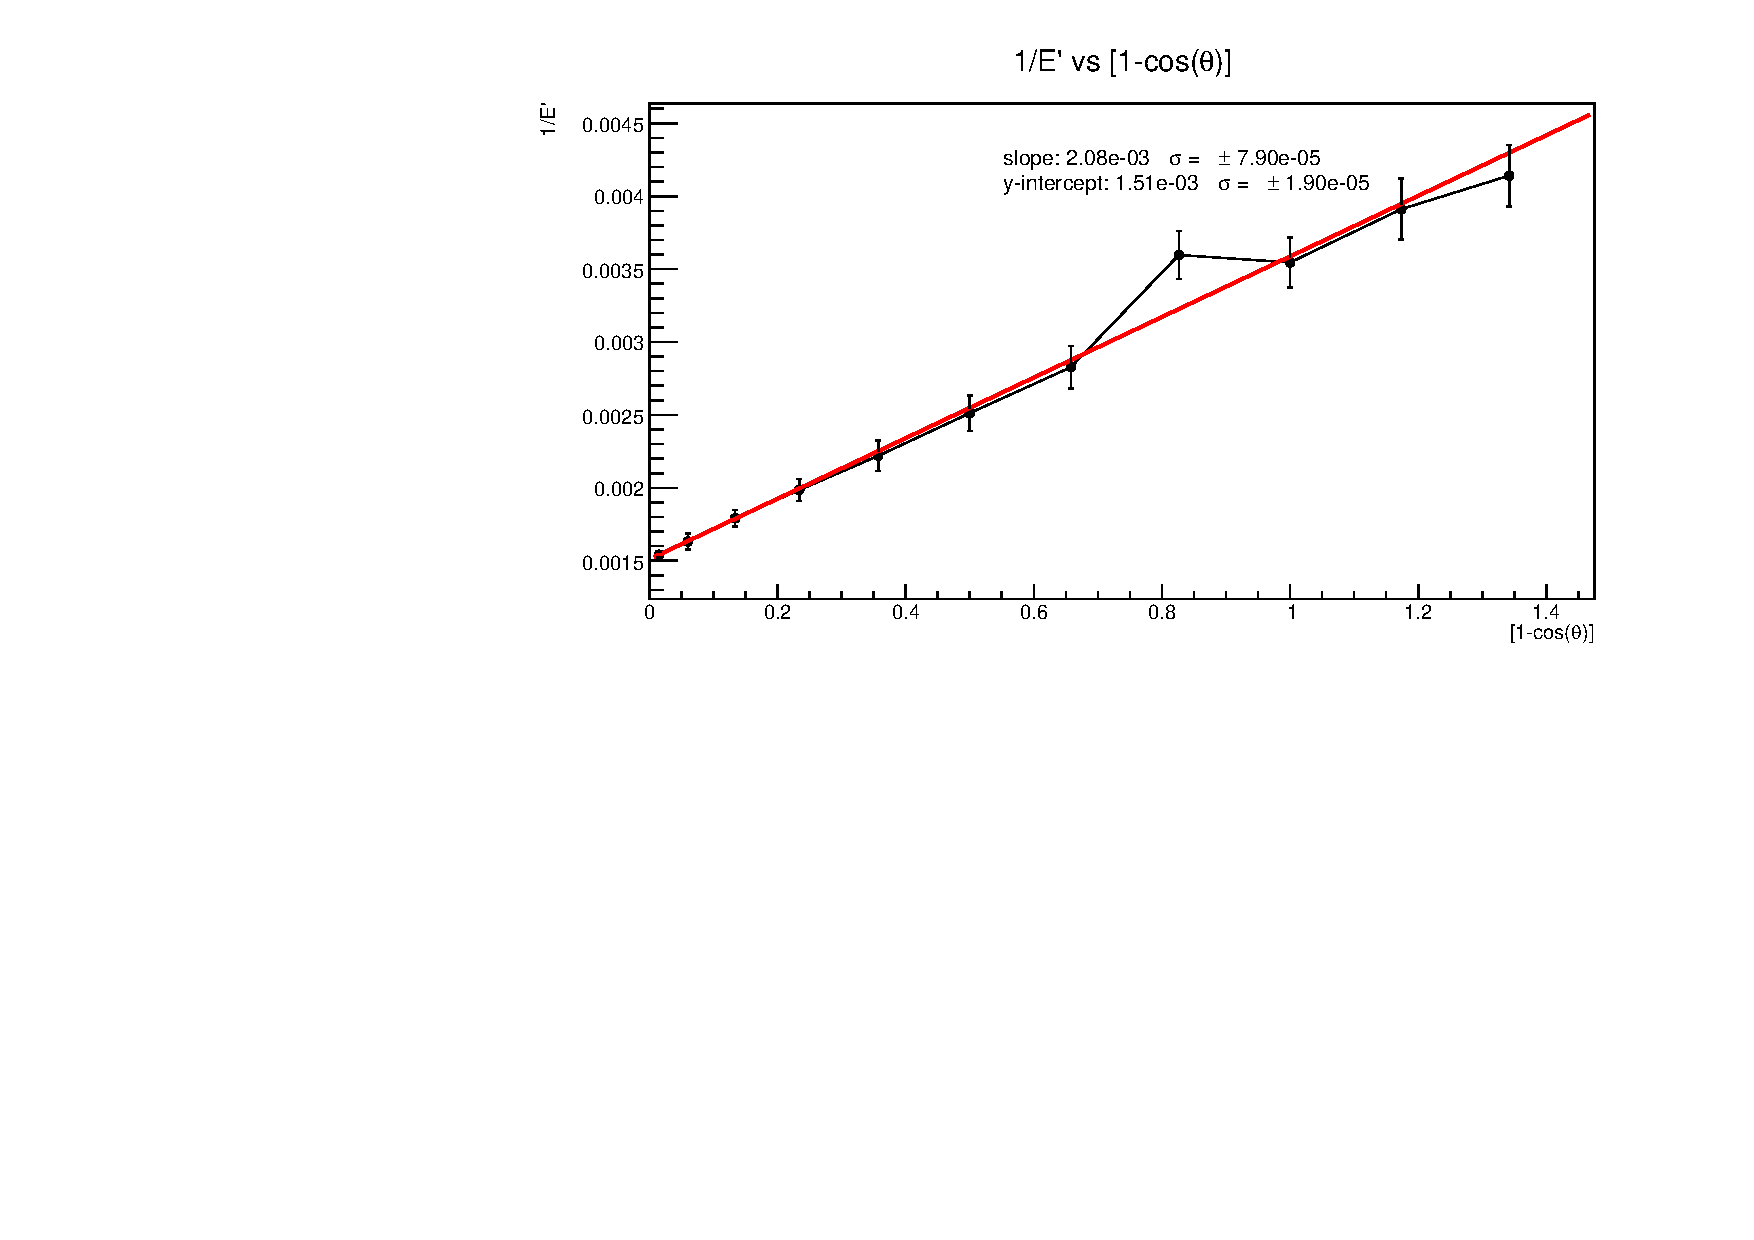
\includegraphics[width=1.0\linewidth]{6-compton/images/COMPTON-DATA.pdf}
    \caption{ The x-axis is 1-cos($\theta$):  $\theta$ represents the angle (relative to the plane of attack) the photon reflects after the collision. The y-axis is 1/E' where E' is the energy of the scattered gamma-ray. The uncertainty in both the slope and y-intercept was calculated due to some complicated formula in ROOT's TF1 class.
    }
    \label{fig:compton-plot}
\end{figure}

\begin{figure}[tbh]
    \centering
    \includegraphics[width=0.9\linewidth]{6-compton/images/Counts vs. Energy (40°).pdf}
    \caption{ This shows a histogram for the energy levels of scattered electrons. In this graph, the detector is set at an angle of 40$^\circ$ relative to the source.
    }
    \label{fig:compton40}
\end{figure}

\begin{figure}[tbh]
    \centering
    \includegraphics[width=0.9\linewidth]{6-compton/images/Counts vs. Energy (50°).pdf}
    \caption{ This shows a histogram for the energy levels of scattered electrons. In this graph, the detector is set at an angle of 50$^\circ$ relative to the source.
    }
    \label{fig:compton50}
\end{figure}



\end{document}